%% LyX 2.0.2 created this file.  For more info, see http://www.lyx.org/.
%% Do not edit unless you really know what you are doing.
\documentclass[12pt,a4paper,english,intoc,bibliography=totoc,index=totoc,BCOR10mm,captions=tableheading,titlepage,fleqn]{scrbook}
\usepackage{lmodern}
\renewcommand{\sfdefault}{lmss}
\renewcommand{\ttdefault}{lmtt}
\usepackage[T1]{fontenc}
\usepackage[latin9]{inputenc}
\usepackage{fancyhdr}
\pagestyle{fancy}
\setcounter{secnumdepth}{3}
\setlength{\parskip}{\medskipamount}
\setlength{\parindent}{0pt}
\usepackage{babel}
\usepackage{calc}
\usepackage{textcomp}
\usepackage{amsmath}
\usepackage{amssymb}
\usepackage{graphicx}
\usepackage[unicode=true,pdfusetitle,
 bookmarks=true,bookmarksnumbered=true,bookmarksopen=true,bookmarksopenlevel=1,
 breaklinks=false,pdfborder={0 0 0},backref=false,colorlinks=false]
 {hyperref}
\hypersetup{
 pdfpagelayout=OneColumn, pdfnewwindow=true, pdfstartview=XYZ, plainpages=false}
\usepackage{breakurl}

\makeatletter

%%%%%%%%%%%%%%%%%%%%%%%%%%%%%% LyX specific LaTeX commands.
\special{papersize=\the\paperwidth,\the\paperheight}

%% Because html converters don't know tabularnewline
\providecommand{\tabularnewline}{\\}

\@ifundefined{date}{}{\date{}}
%%%%%%%%%%%%%%%%%%%%%%%%%%%%%% User specified LaTeX commands.
% increase link area for cross-references and autoname them
\AtBeginDocument{\renewcommand{\ref}[1]{\mbox{\autoref{#1}}}}
\newlength{\abc}
\settowidth{\abc}{\space}
\AtBeginDocument{%
\addto\extrasenglish{
 \renewcommand{\equationautorefname}{\hspace{-\abc}}
 \renewcommand{\sectionautorefname}{sec.\negthinspace}
 \renewcommand{\subsectionautorefname}{sec.\negthinspace}
 \renewcommand{\subsubsectionautorefname}{sec.\negthinspace}
 \renewcommand{\figureautorefname}{Fig.\negthinspace}
 \renewcommand{\tableautorefname}{Tab.\negthinspace}
}
}

% in case somebody want to have the label "equation"
%\renewcommand{\eqref}[1]{equation~(\negthinspace\autoref{#1})}

% that links to image floats jumps to the beginning
% of the float and not to its caption
\usepackage[figure]{hypcap}

% the pages of the TOC is numbered roman
% and a pdf-bookmark for the TOC is added
\let\myTOC\tableofcontents
\renewcommand\tableofcontents{%
  \frontmatter
  \pdfbookmark[1]{\contentsname}{}
  \myTOC
  \mainmatter }

% make caption labels bold
\setkomafont{captionlabel}{\bfseries}
\setcapindent{1em}

% enable calculations
\usepackage{calc}

% fancy page header/footer settings
\renewcommand{\chaptermark}[1]{\markboth{#1}{#1}}
\renewcommand{\sectionmark}[1]{\markright{\thesection\ #1}}

% increase the bottom float placement fraction
\renewcommand{\bottomfraction}{0.5}

% avoid that floats are placed above its sections
\let\mySection\section\renewcommand{\section}{\suppressfloats[t]\mySection}

\makeatother

\begin{document}



\subject{Seminar Report}


\title{Dynamic Decentralized Mapping on NoC Architectures}


\author{Apoorv Kumar}


\date{09010111}


\publishers{%
\framebox{\begin{minipage}[t]{0.4\columnwidth}%
%
\end{minipage}}\vspace{\baselineskip}\\
Department of\\
Computer Science \& Engineering\\
Indian Institute of Technology - Guwahati\vspace{-3cm}
}


\lowertitleback{\textbf{Guiding Professor}\smallskip{}
\\
Dr. Hemangee Kapoor\bigskip{}
\bigskip{}
\\
}


\dedication{Where the ENIAC is equipped with 18000 vacuum tubes and weighs 30
tons , computers in future may have only 1000 vacuum tubes and weigh
only 1.5 tons. {\small - Popular Mechanics , 1944}}

\maketitle
\pagebreak{}


\lhead{\rightmark}


\rhead[\leftmark]{}


\lfoot[\thepage]{}


\cfoot{}


\rfoot[]{\thepage}

\tableofcontents{}

\newpage{}

\pagestyle{plain}


\chapter*{Introduction}

\addcontentsline{toc}{chapter}{Abstract} 

Intel projects the availability of 100 billion transistors on a 300mm
die by 2015. This allows to integrate thousands of processors or equivalent
logic gates on a single die. Unfortunately , we have hit various roadblocks
on our way to performance enhancement. Heat wall , synchronization
problem , crosstalk at sub-20nm levels , all equally fatal. This forces
us to look towards horizontal rather than vertical scaling. We use
many transistors to increase the working units, rather than improving
one unit. The major challenge lies in trying to map our applications
initially designed for serial execution on these massively parallel
machines. Further since our computers need to handle dynamic loads
, dynamic mapping comes out as the natural preference for mapping.

On-chip packet-switched network have been proposed as a solution for
the problem of global interconnect in deep sub-micron VLSI Systems
on Chip (SoC). Networks on Chip (NoC) can address and contain major
physical issues such as synchronization, noise, error correction and
speed optimization. NoC can also improve design productivity by supporting
modularity and reuse of complex cores, thus enabling a higher level
of abstraction in architectural modeling of future systems .

In this report we discuss the various paradigms available for running
real life applications on the NoC architectures. First we highlight
the compulsions that forced us to switch from the currently prevalent
architectures. Then we justify why we set aside other alternative
architectures in favour of the network based onces. Once we are on
firm footing as to why we have chosen the aforementioned paradigm
, we discuss the parameters that define scalability ,  low cost and
good performance. Further we discuss in details how we plan to run
our applications on the many-cores , that don't nearly resemble the
bus-based architecture we are so used to program for. We show how
centralized mapping has very binding limitations , and that decetralized
mapping is the best way for the distant future. 


\pagebreak{}

\pagestyle{fancy}


\lhead[\chaptername~\thechapter]{\rightmark}


\lhead[\chaptername~\thechapter]{\rightmark}


\rhead[\leftmark]{}


\lfoot[\thepage]{}


\cfoot{}


\rfoot[]{\thepage}


\chapter{Why NoCs / Cost Considerations.}


\section{Overview}

Before we can start on the best/optimal architecture we have to specify
on what grounds we would be measuring performance. Further we have
to ensure that the NOC architecture does improve upon alternative
architectures on these grounds.

Under most widely accepted norms , we analyze the generic cost in
terms of area and power. 

NoCs help us overcome the common issues faced by currently used architectures.
This chapter discusses the problems in brief.


\section{Power}

Power has become the most critical constraint in the design of many
systems, from high-performance servers to em- bedded battery-operated
devices. Recognizing the need to target increasing power consumption
and design complexity in these systems, designers have turned to multi-core
architectures such as chip multiprocessors (CMPs) and multiprocessor
systems-on-a-chip (MPSoCs).


\subsection{Network Power}

Both the processor cores as well as the NoC communication fabric can
be modeled as a fully connected directed graph \textit{\small G =
(N, L)} where N is the set of nodes and L is the set of links in G.
This holds true for the ordinary multi-processors as well , and uni-cores
just behave as a trivial subset. The only difference lies in how the
fabric behaves. Whereas in unicores this power can be safely neglected
, this power is included in the shared-bus power consumption for the
ordinary multicores.

There are many frameworks for the estimation of this power. Some of
them being LUNA and Orion.

Most commonly used ``proxy-parameters'' for the power consumption
include link-utilization. Dynamic network power, is a function of
activity/utilization and energy costs (constants) for each of the
key router components. Using link utilization as an abstraction for
network power , the level of activity at a network link is used as
a measure the overall power consumption of that network router and
link.\cite{Eisley:2004:HPA:1023833.1023849}


\subsection{Processor Power }

Since we can model the processor cores using the same above graph,
the same frameworks would work fine here as well. But in contrast
to the network model , the data transfer over nodes is much cheaper
and faster process. Resource utilization is usually used as a proxy
for power, similar to the way we abstract network power through link
utilization in Section 1.2.1, we abstract the power consumption of
a processor by the utilizations of individual resources. The summation
of the energy costs of each component (functional units, register
file, caches etc.) is captured by each respective utilization function. 

In the case of the network fabric, the utilization of all of the components
is approximately equal because message flowing in networks consume
roughly the same amount of energy per hop. Estimates of individual
network components\textquoteright{} energy consumptions are thus not
necessary because it is a relative power measure; constant factors
can be eliminated. However, in the case of a processor pipeline, each
instruction will not consume the same amount of energy. The component
utilizations hence cannot be removed and abstracted as a single utilization.
Relative estimates are thus required in order to obtain a relatively
accurate estimation of processor power.


\section{Area}

With the failure of Dennard scaling and thus slowed supply voltage
, scaling core count scaling may be in jeopardy, which would leave
the community with no clear scaling path to exploit continued transistor
count increases. In any case , preserving the transistors for the
purpose of actual computing is a priority for any designer.For instance,
by increasing the buffer size at each input channel from 2 to 3 words,
the router area of a 4x4 NoC increases by 30\% or more\cite{Ogras:2005:KRP:1084834.1084856}.To
this end we like to keep the buffers (that add absolutely nothing
to computations) to the minimum.Buffer consumes much of silicon and
power and this is likely to reduce performance. 



\lhead[\chaptername~\thechapter]{\rightmark}


\rhead[\leftmark]{}


\lfoot[\thepage]{}


\cfoot{}


\rfoot[]{\thepage}


\chapter{A comparison of various architectures}


\section{Overview}

Multicores and Systems on Chip (SoCs) require efficient inter-module
interconnection providing for the required communications at a low
cost. Using the previously defined costs , using area and power we
would try to analyze how the different architectures fare : a shared
bus, a segmented bus and a point-to-point interconnect. For each architecture
we discuss analytical expressions for area, power dissipation and
operating frequency as well as asymptotic limits of these functions. 

We show how NoCs actually provide scalability advantages over other
architecture and thus are better prospects for the future. While the
costs associated with a chip is measured in terms of power and area
, the most commonly accepted measure of performance is QoS. QoS is
usually associated with throughput and latency. 


\section{NoC topology}

We assume a very basic mesh network topology for the NoCs discussed.


\subsection{NoC communication fabric}

Packets carry routing information, command and payload. While the
payload delivers the real data , some overhead is unavoidable , akin
to the large scale networks. The command field identifies the payload,
specifying the type of operation. The packet is divided into multiple
flits following . Flit transfer over the inter-router link may be
controlled by handshake. 


\subsection{NoC routers}

NoC comprises routers interconnected by point-to-point links. Network
topology can vary depending on system needs and module sizes and placement.
Each system module is connected to a router (Fig. 1) via a standard
interface, whose bandwidth might be adapted to the communication needs
of that module. The bandwidth of each inter-router link is similarly
adjusted to accommodate the expected traffic and fulfill QoS requirements
at the specific link. The link bandwidth can be controlled by the
link frequency and link width.

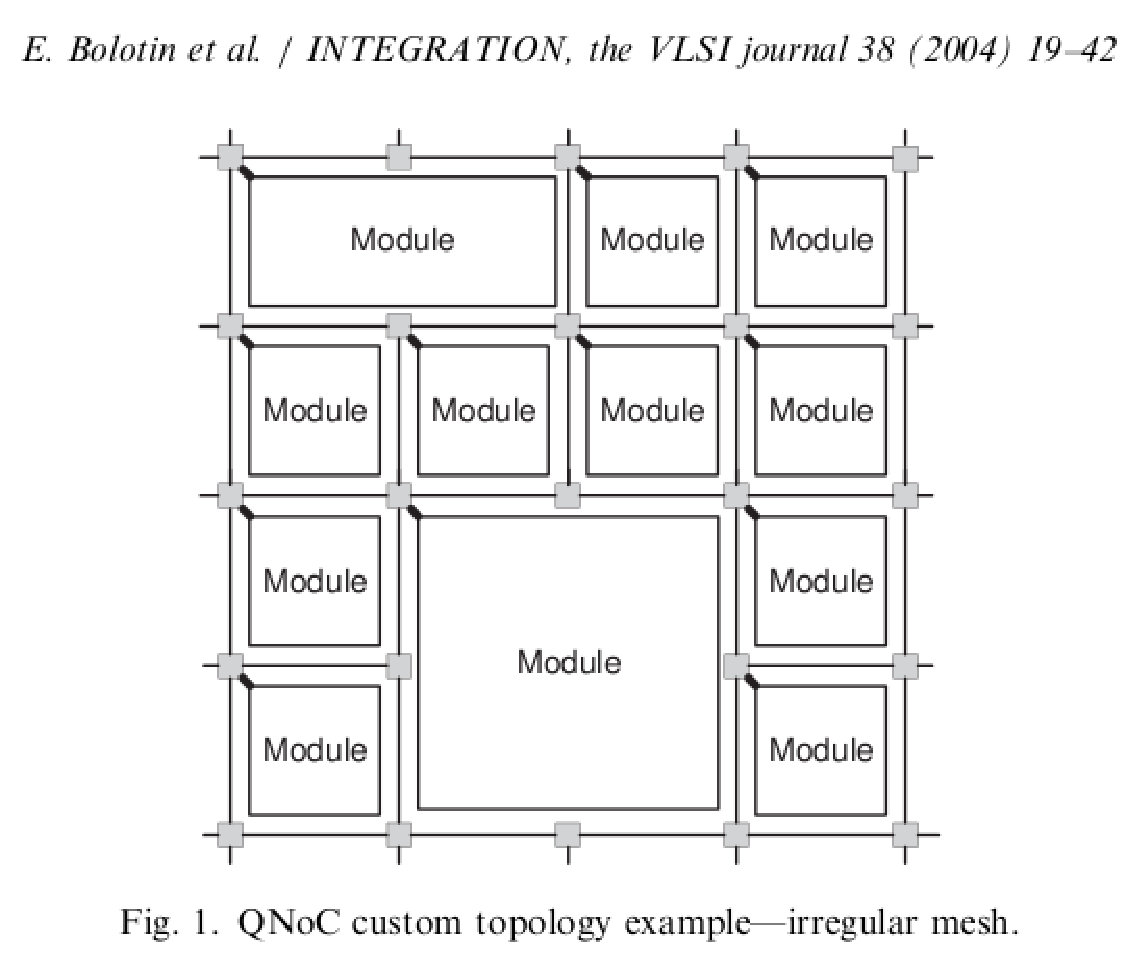
\includegraphics[width=7cm]{images/1}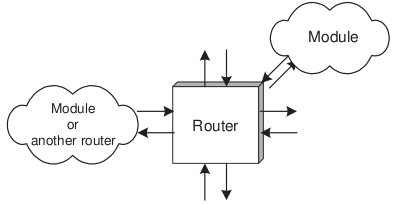
\includegraphics[scale=0.4]{images/2}


\subsection{NoC IPs}

The IPs consist of the functional part of NoC that is directly involved
in computations. It may be a memory module , a generic processor or
a special purpose processor. The variety of IP cores is as wide as
that of in SoCs.


\section{Cost Comparisons}


\subsection{Various Topolgies}


\subsubsection{NoC}

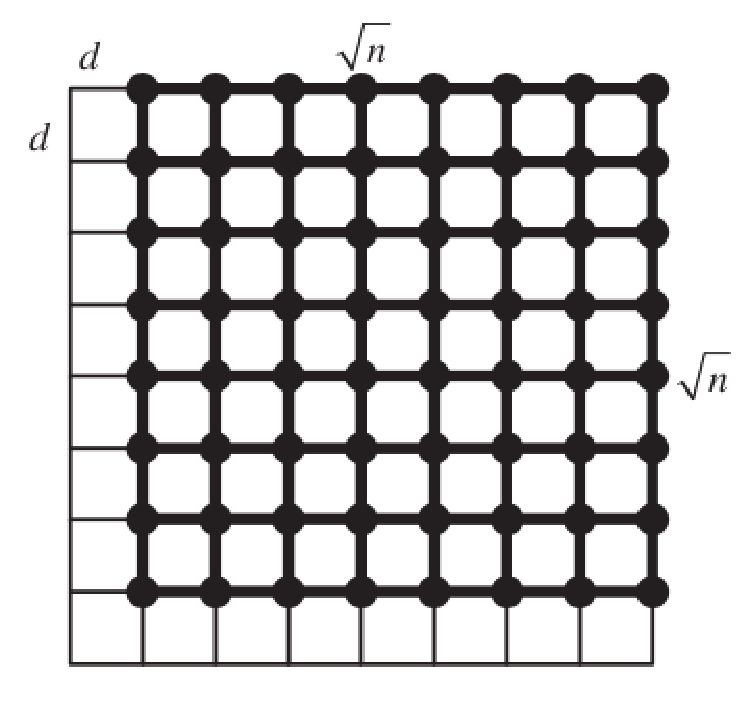
\includegraphics[width=7cm]{images/3}\cite{Bolotin:2004:CCN:1056481.1056484}%
\framebox{\begin{minipage}[t]{0.1\columnwidth}%
Fig. 2%
\end{minipage}}

Consider n system modules interconnected by a NoC (Fig. 2). Each module
is connected to a router using a standard interface, and the routers
are interconnected in a mesh topology. For the NoC case, we assume
that the silicon cost of minimal buffer routers and simple module
interfaces are comparable to similar costs of other solutions (such
as bus multiplexers, bus interfaces, etc.). Moreover, these costs
are linear with the number of modules and therefore do not change
the asymptotic comparison. 


\subsubsection{Unsegmented Bus}

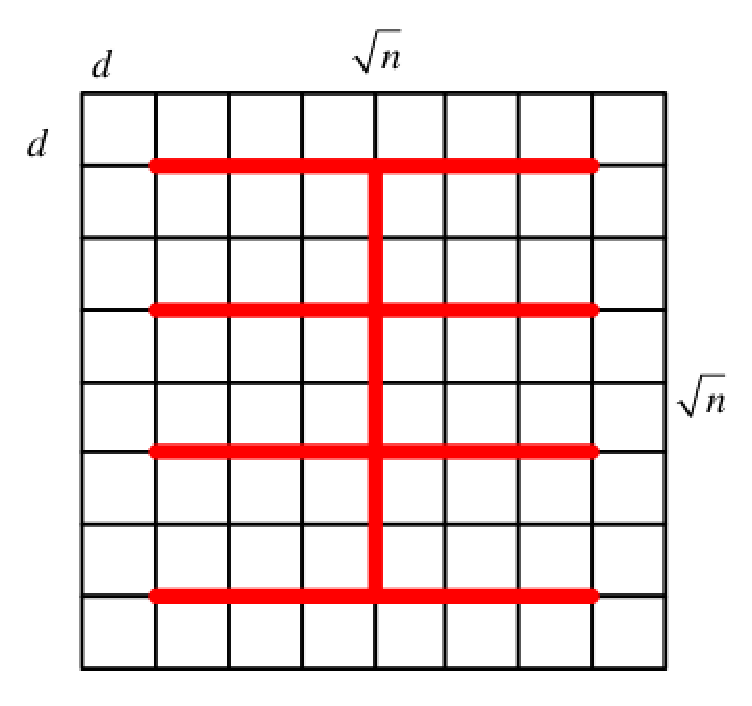
\includegraphics[width=7cm]{images/4}\cite{Bolotin:2004:CCN:1056481.1056484}%
\framebox{\begin{minipage}[t]{0.1\columnwidth}%
Fig. 3%
\end{minipage}}

The NS-Bus is a simple shared bus, connecting all modules in the system
and laid out as a minimal spanning tree (Fig. 3). It consists of a
single segment and has no parallelism (only one transaction is active
at a time). 


\subsubsection{Segmented Bus}

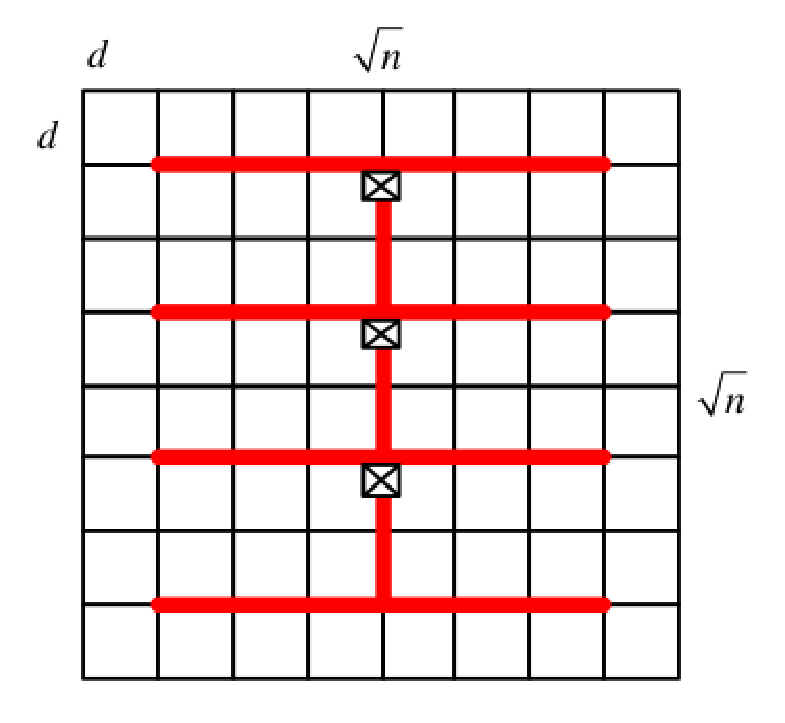
\includegraphics[width=7cm]{images/5}\cite{Bolotin:2004:CCN:1056481.1056484}%
\framebox{\begin{minipage}[t]{0.1\columnwidth}%
Fig. 4%
\end{minipage}}

The S-Bus is the most widely used SoC interconnection architecture,
primarily because a long shared bus that interconnects all system
modules is not feasible in systems consisting of many communicating
nodes. We assume a similar topology as NS-Bus, but segmented into
n/2 identical sections (of the same length, width and frequency).
The interconnection is established by bridges, as in Fig. 4. The S-Bus
has more parallelism, because the segments are independent. Also,
the capacitance of each segment is substantially reduced relative
to that of the NS-Bus, allowing the S-Bus to operate at higher frequencies.
This structure was a deviation from the primitive single bus architectures
, and a move towards the connection based ones.


\subsubsection{Point to Point}

Consider n modules arranged in a mesh and interconnected point-to-point
with links that are routed in an X-Y fashion, similar to the NoC.
Note that here , the wires are routed instead of packets. This has
the direct implication that the net wire length explodes with the
network size. We are forced to resort to such an architecture because
the 2D chips enforce a constraint of planarity of topology (ie the
wires cannot intersect). The view of network is exactly same as that
of Fig 2.


\subsection{Asymptotic Bounds}

Following the aforementioned specifications \cite{Bolotin:2004:CCN:1056481.1056484}
arrived at the following asymptotic complexities.

\begin{tabular}{|c|c|c|c|}
\hline 
Architecture & Total Area & Power dissipation & Operating frequency\tabularnewline
\hline 
\hline 
NS - Bus & O($n^{3}\sqrt{n}$) & O($n\sqrt{n}$) & O($\tfrac{1}{n^{2}}$)\tabularnewline
\hline 
S - Bus & O($n^{2}\sqrt{n}$) & O($n\sqrt{n}$) & O($\tfrac{1}{n}$)\tabularnewline
\hline 
NoC & O($n$) & O($n$) & O(1)\tabularnewline
\hline 
PTP & O($n^{2}\sqrt{n}$) & O($n\sqrt{n}$) & O($\tfrac{1}{n}$)\tabularnewline
\hline 
\end{tabular}

\ \\

The total area: 
\begin{itemize}
\item Since the NS-bus operates at a very slow frequency (decreasing as
O($\tfrac{1}{n^{2}}$) ) and has no parallelism, it has to be made
excessively wide to provide the same effective in order bandwidth
as the NoC.As a result, its width grows as O($n^{2}\sqrt{n}$) and
its length grows as O($n$), so that its total area cost function
grows as O($n^{3}\sqrt{n}$)
\item The S-Bus is O($n$) faster than the NS-Bus because each segment is
O($n$) shorter and it employs O($n$) segments in parallel, but since
the average number of hops traversed on the segmented bus is also
O($n$) ; it results in no parallelism. Thus, the S-bus requires O($n$)
fewer links than the NS-bus and its total area cost function is O($n^{2}\sqrt{n}$)
\item The NoC wire-cost increases only as O($n$)
\item In PTP the average link frequency O($n$) slower than in the NoC (longer
links with higher capacitance).
\item The, link length grows as O($n^{2}\sqrt{n}$) and since the link width
is asymptotically O(1), its total area also grows as O($n^{2}\sqrt{n}$)
\end{itemize}
\ \\

The power dissipation cost function:
\begin{itemize}
\item Power dissipated by all architectures is proportional to the product
of operating frequency and total wire length. 
\end{itemize}
\ \\

Thus , our analysis clearly shows an asymptotic supremacy of the NoC.
Our assumptions being, a uniform traffic distribution and assuming
that load capacitance depends only on the interconnect (ignoring the
capacitance of system module ports). It is notable that the above
assumptions only put NoC on the lower ground. Non uniform traffic
, mostly local, favours NoC , as does the inclusion of port capacitance.
As the technology improves, NoC is the only communication architecture
where the links become shorter and less vulnerable to delays and noise. 







\lhead[\chaptername~\thechapter]{\rightmark}


\rhead[\leftmark]{}


\lfoot[\thepage]{}


\cfoot{}


\rfoot[]{\thepage}


\chapter{Performance parameters and QoS on NoCs.}


\section{Overview}

In this section we discuss Quality of Service (QoS) for communications
in Systems on Chip (SoC), as the minimum guarantees provided on the
associated parameters. SoC inter-module communication traffic can
be classified into four basic classes of service: signaling, real-time,
RD/WR and block-transfer .

As we have already seen , latency, throughput and reliability are
the most widely accepted parameters to be considered when talking
about QoS. Communication traffic of the target SoC can be analyzed
by means of analytic calculations and simulations, and QoS requirements
(delay and throughput) for each service class can be accordingly derived.
In this section we analyze how we can conform to a QoS.


\section{Class based traffic}

We have different types of traffic. Some are bound by strict time,
delay and reliability constraints, while others are not of much importance
and can be done at liesure. Thus in order to quantize QoS levels and
check for conformity , we need to categorize the traffic into 4 broad
groups.\cite{Bolotin:2004:QQA:985396.985400}
\begin{enumerate}
\item \textbf{Signaling} covers urgent messages and very short packets that
are given the highest priority in the network to assure shortest latency.
This service level is suitable for interrupts and control signals
and alleviates the need for dedicating special, single-use wires for
them. 
\item \textbf{Real-Time }service level guarantees bandwidth and latency
to real-time applications, such as streamed audio and video processing. 
\item \textbf{Read/Write (RD/WR)} service level provides bus semantics and
is hence designed to support short memory and register accesses. 
\item \textbf{Block-Transfer} service level is used for transfers of long
messages and large blocks of data, such as cache refill and DMA transfers. 
\end{enumerate}

\section{Parameters}


\subsection{Latency}

Latency is defined as the precursor time to the actual start of data
transfer. This includes the time consumed for connection establishment
and propogation delay.

Store-and-forward routing techniques come out as big culprits in assuring
low latency. Besides incurring high buffer requirements , they are
subject to huge queing delays, as a router waits for next router to
have enough free buffer. 

Circuit switching is not an option if we are to maintain a constrained
latency. Though the service after a connection is made can be better
than any other option, the wait while a dedicated path is established
can be a long one. Further this leads to poor resource utilization.
Since in order delivery is of great importance to us , we find a suitable
replacement in virtual-circuit switching. The connection establishment
is rather quick , and decent guarantees can be made once the connection
is established.

Wormhole routing reduces latency and buffer requirements in the routers.
It combines virtual cut-through with small unit size and is a currently
accepted solution for providing latency gurantees. In wormhole switching,
a packet is transmitted between the nodes in units of flits, the smallest
units of a message on which flow control can be performed. The header
flit(s) of a message contains all the necessary routing information
and all the other flits contain the data elements. The flits of the
message are transmitted through the network in a pipelined fashion.
Since only the header flit(s) has the routing information, all the
trailing flits follow the header flit(s) contiguously. \cite{Mohapatra:1998:WRT:292469.292472}


\subsection{Throughput}

Throughput is defined as the maximum theoretical rate of data transfer
over the network.

Though cirtuit switching can provide best throughput guarantees ,
it is avoided due to the high cost of establishing and managing circuit
connections along with poor resource utilization. This is in contrast
with the completely connection less data transer , which better utilizes
the hardware , but is prohibitory considering the silicon spent on
re-ordering buffers.

So we arrive at a trade-off , and choose a hybrid technique. Virtual
cut through (as has been discussed earlier) solves the constraints
of being plausible , efficient and reliable.





\lhead[\chaptername~\thechapter]{\rightmark}


\rhead[\leftmark]{}


\lfoot[\thepage]{}


\cfoot{}


\rfoot[]{\thepage}


\chapter{Application Mapping on NoCs}


\section{Overview}

NoCs (or SoCs in general) are being developed to improve the computational
acumen at our disposal. We want better performance ( that can be associated
to QoS) for real life applications such as word processors , media
players and high-end graphics. This leads us to our next problem.
How to map the applications, that were previously trivially implemented
as serial, on a many-core. Unfortunately it turns out that all task
allocation problems for NoCs can be modeled as bin-packing problem
( a NP complete problem ) . 

Fortunately , it isn't the end of it. There are efficient algorithms
that give decent allocation results in practice. Further , though
the allocation of tasks on processors can be reduced to bin packing,
we also need to pay attention to minimizing communication.

Thus we are faced with a tradeoff.

Linear clustering , targets close allocation of communicating processes
and leads to lower communication , but may lead to worse utilization
or processing power.

Efficient bin packing may increase communication overhead, but gives
better utilization.

This section discusses the various mapping strategies that are avaible
to us.

\pagebreak


\section{Mapping Paradigms}

We need to map the tasks , applications and IP cores into equivalent
mathematical entities that can in turn be mapped into each other and
analyzed for performance. Most researchers use two standard mathematical
tools that are solve the purpose well.\cite{Ogras:2005:KRP:1084834.1084856}
\begin{enumerate}
\item \textbf{Communication Task Graph} (CTG) G\textasciiacute{} = G\textasciiacute{}
( T, D ) is a directed acyclic graph, where each vertex represents
a computational module in the application referred to as task $t_{i}\in T$
. Each task $t_{i}$ is annotated with relevant information, such
as execution time on each type of Processing Element (PE) in the network,
task i energy consumption ( $e_{j}^{i}$ ) when executed on the j-th
PE, individual task deadlines ( $dl(t_{i})$ ), periodicity of the
task graphs, etc. Each directed arc $d_{i,j}\in D$ between tasks
$t_{i}$ and $t_{j}$ characterizes either data or control dependencies.
Each $d_{i,j}$ has associated a value $v(d_{i,j})$ , which stands
for the communication volume (bits) exchanged between tasks $t_{i}$
and$t_{j}$ . 
\item \textbf{Application Characterization Graph} (APCG) G = G ( C, A )
is a directed graph, where each vertex $c$ $i\in C$ represents a
selected IP/core, and each directed arc $a_{i,j}$characterizes the
communication process from core $c_{i}$ to core $c_{j}$ . Each $a_{i,j}$
can be tagged with application-specific information (e.g. communication
volume, communication rate, etc.) and specific design constraints
(e.g. communication bandwidth, latency requirements, etc.). Also,
the size/shape of cores $c_{i}\in C$ is assumed to be known. 
\end{enumerate}

\subsection{Static Mapping}

Static mapping paradigm dictates developing NoC platforms where both
computation and communication have been pre-designed. Since such platforms
offer no real flexibility for architectural customization, the mapping
issue reduces to solving the communication and task scheduling problems.
Although the scheduling problem is a traditional topic in computer
science, the interprocessor communication gives it a new flavor altogether. 

The static mapping can be formalized using the 2 tools we discussed
previously. \cite{Ogras:2005:KRP:1084834.1084856}

ACG can be uniquely described by the 4-tuple $\text{\ensuremath{H}}(C,A(R,Ch),\Re,\Omega(C))$

$C$- represents the set of cores/PEs.

$A(R,Ch)$ - is a directed graph and describes the communication infrastructure;
the routers $(R)$ and the channels $(Ch)$ in the network have attributes
such as, $\forall(ch)\in Ch$ , $W(ch)$ gives the width of the network
channels $\forall r\in R,\; l(d,r)$ gives the input buffer size (depth)
for the communication port d at router $r\in R$ . $\forall r\in R,\: P(r)$
specifies the position of the router $r$. 

$R(RD(r,s,d,\rho(n)),Sw)$- describes the communication paradigm adopted
in the network. 

$RD(r,s,d,\rho(n)),s,d,r\in R,n\subseteq R$ defines the routing policy
at router $r$ for all packets with source $s$ and destination $d$.
In this function, $\rho(n)$ denotes the utilization of the neighboring
routers, which can be used by an adaptive algorithm. Finally, $Sw$
specifies the packet switching technique implemented in the network. 

$\Omega:C\rightarrow R$ - maps each core $c_{i}\in C$ to a router.
For direct topologies, each router is connected to a core, while in
indirect topologies some routers are connected only to other routers. 

We can regard the architectural choices in the design of NoCs as representing
a 3D design space, where each component of the triple $H'(A(R,Ch),R,\Omega(C))$
defines a separate dimension. In the design automation community,
design space exploration along each dimension has been performed to
some extent without explicitly considering such a formalism. 

The algorithms that target real-time or DSP applications where the
worst-case task execution time and inter-task communication volume
are pre-characterized can be modeled as CTGs which expose the inherent
inter-node parallelism existing in the application. 


\subsection{Dynamic Mapping}

Static mapping gives encouraging results for application specific
domains , however, such a fully static scheduling, can not be directly
applied to applications containing conditional branches. As is the
case with general purpose computing when applications behavior can
not be predicted at compile time, on-line scheduling approaches are
usually needed. This gives us the inspiration to develop a dynamic
version of the mapping process.

Dynamic Mapping may still be divided into centralized and decentralized.
Whereas sufficient research work has been on the centralized methods
, decentralized techniques still remains largely unexplored , more
so because of the complexities involved. It is often implausible to
let the application graph expand without keeping track of it , and
expect it to be doing precisely what it was supposed to. Very application
specific developments have been made in this field. One being decentralized
mapping for tree-structured applications , which will be discussed
in depth in the dedicated next chapter.


\subsubsection{Mapping Strategies}

Before we analyze the dynamic mapping methods , let us analyze the
ways in which we can constrain partitioning the graph so we have least
number of regions to analyze (thus reducing administrative overhead)
, and most accurate administration. This usually happens by limiting
the ways in which resources are allocated to the jobs. Since administration
comes into picture , these are almost always used by centralized mapping
methods , most likely administered by the master node (running OS).

When analyzing the communication between nodes , we come across 2
types of messages:
\begin{enumerate}
\item Intra-process
\item Inter-process
\end{enumerate}
These further give rise to 2 types of contentions as shown in Fig.
6
\begin{enumerate}
\item Internal contention - contention that arises due to nodes processing
the same job vying for a link.
\item External contention - contention that arises due to nodes processing
separate jobs vying for a link.
\end{enumerate}
Any good resource allocation mechanism would seek to minimize these
contentions , and maximize resource utilization. It is seen that the
contiguous allocation strategy achieves only 34\textendash{}66\% resource
utilization, while the non-contiguous allocation strategies can reach
up to 78\%. However, the performance of non-contiguous allocation
may suffer due to internal and external contention.

\includegraphics[scale=0.6]{images/image}%
\framebox{\begin{minipage}[t]{0.2\columnwidth}%
Fig. 6\cite{Chou:2008:UDT:1403375.1403675}%
\end{minipage}}

\ \\


\subparagraph{Contiguous resource allocation}

Fig 6.a

Resources are allocated such that they form a convex shape and are
closely packed. This method reduces the external contention , but
has high internal contention. If we assume that intra process messages
are more frequent than inter process , then this leads to lower hops
per message. Unfortunately , this can lead to segmentation and after
a while , a process might not get sufficient processors because they
are not contiguous. This implies lower resource utilization.


\subparagraph{Random resource allocation}

Fig 6.b

Resources are allocated randomly. Leads both high internal and external
contention. In complete contrast to contiguous resource allocation
, this leads to higher hops per message but better resource utilization.
Poor latency and throughput make is least favoured.


\subparagraph{Paged resource allocation}

Fig 6.c

In this method , resources are divided into sections called pages.
Any process can get only a multiple of 1 page , irrespective of it's
requirements.\textquotedblleft{}Paging\textquotedblright{} selects
the non-allocated sub-meshes in row-major order. But it , on one hand
betters the resource utilization because the segmentation is eliminated
, on the other hand worsens it , since some resource might go waste
inside each page. 


\subparagraph{MBS resource allocation}

Fig 6.d

multiple buddy strategy (MBS) the mesh network is initially divided
into nonoverlapping sub-meshes. In contrast to paging , \textquotedblleft{}MBS\textquotedblright{}
allocates jobs to contiguous sub-meshes if possible.


\subparagraph{GABL resource allocation}

Fig 6.e

\textquotedblleft{}greedy\textendash{}available\textendash{}busy\textendash{}list
(GABL)\textquotedblright{} allocates the resources from the largest
free sub-mesh of any size. 


\subsubsection{Centralized Mapping}

Centralized mapping procedures have, in common, the feature that a
master node acts as a moderator and administrator of tasks. The central
node handles re-assignment of applications when necessary or assignment
of new applications to nodes. This , though has sufficient pedagogical
backing in terms of text , is not scalable to very large number of
IP cores. Primary reasons behind this are
\begin{enumerate}
\item the generation of a hot-spot - all nodes try to send data to the central
node.
\item explosion of data to be processed by central node - total data to
be processed increases linearly with total number of cores. With the
number of cores likely to scale with the transistors , this happens
to be exponential.
\end{enumerate}
Mapping the tasks onto hardware can include 2 procedures:
\begin{enumerate}
\item Allocating jobs to free IPs/resources.
\item Migrating/reclustering the previously allocated jobs to create space
for the new job.
\end{enumerate}
While the first option is fast and found across all NoCs , the second
is very time consuming and not commonly implemented. Migration of
a already embedded task pays off only if the program is destined to
run for a very long duration, and thus the added efficiency more than
compensates for the migration overhead. 

We discuss some of the centralized mapping techniques below.


\paragraph{User Behaviour based - }

For application-specific NoCs, the design methodologies proposed so
far solve various problems (e.g., task mapping, link scheduling) off-line,
in a static manner. However, for multiple use-case NoCs which deliver
high performance computing for embedded pplications), different system
configurations resulting from multi-user behavior are too dynamic
and too complex in nature to be modeled off-line. \cite{Chou:2008:UDT:1403375.1403675}

\includegraphics[width=15cm]{images/image}%
\framebox{\begin{minipage}[t]{0.2\columnwidth}%
Fig. 7\cite{Chou:2008:UDT:1403375.1403675}%
\end{minipage}}

Mapping techniques focus at:

1) maximizing the utilization of system resources

2) maximizing jobs performance. 

But since these two are often conflicting , and the best choice of
resource allocation scheme (from the 5 discussed in 4.2.2.1) is not
static. The master node has 3 options :

1) Approach 1: (Fig 7.c) Focus on minimizing the internal contention
and communication cost; minimize the external contention only as a
secondary goal.

2) Approach 2: (Fig 7.d) Focus on minimizing the external contention;
minimize the internal contention and communication cost only as a
secondary goal. 

3) Hybrid approach: (Fig 7.e) A hybrid method consists of combining
Approaches 1 and 2 while taking user behavior into consideration. 


\paragraph{Agent based - }

This is a hierarchical method wherein we create cluster agents to
monitor the members of that cluster. \cite{4555921}.

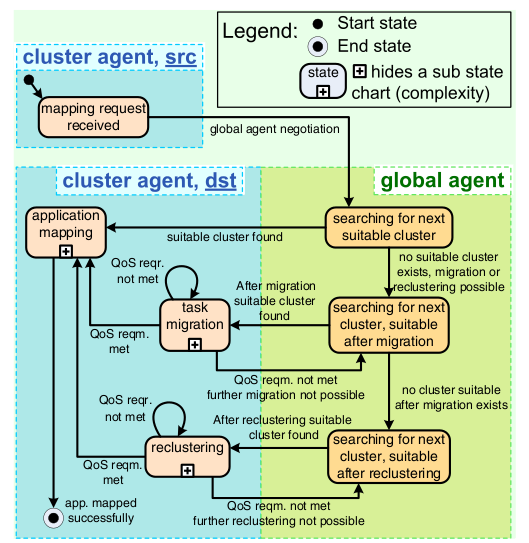
\includegraphics[width=10cm]{images/6}%
\framebox{\begin{minipage}[t]{0.2\columnwidth}%
Fig. 8\cite{4555921}%
\end{minipage}}

The run-time mapping in such a scheme is achieved by using a negotiation
policy among Cluster Agents (CAs) and Global Agents (GAs) of a certain
instance of time distributed over the whole chip. In Fig. 8 an application
mapping request is sent to the CA of the requesting cluster which
receives all mapping requests and negotiates with the GAs. There can
be multiple instances of the GAs that are synchronized over time.
The GAs have global information about all the clusters of the NoC
in order to make decisions onto which cluster the application should
be mapped to. Possible replies to this mapping request are: 

1. When a suitable cluster of the application exists then the GAs
inform the requesting source CA and the requesting source CA asks
the suitable destination CA for the actual mapping of the application. 

2. When no suitable clusters are found by the GAs then the GAs report
the next most promising cluster where it is possible to map the application
to after task migration which is negotiated between the GA and the
CA to make this cluster suitable for the mapping. The number of iterations
is a configuration parameter. 

This is targeted at reducing the problem of hotspot , by making decisions
at a lower level. The communication of agents with the global agent
is sparse and thus reduces the overhead traffic, along with the associated
congestion.


\paragraph{Incremental Mapping}

Chou et al \cite{4627545} proposed an incremental mapping scheme
that is performance aware and takes into account the possiblity of
scheduling of new jobs. They suggest a new cluster selection called
near-convex region cluster. They assume a central manager and separate
control network.

\includegraphics[width=7cm]{images/image}\includegraphics[width=8cm]{images/image}

As such, all the previous works mentioned earlier do not maximize
the system efficiency by considering the possible addition of new
applications and NoC-based communication.They claim to optimize the
communication energy consumption for all possible system configurations
(at different time instances), considering that applications can dynamically
arrive and leave the system. 


\subsubsection{Decentralized Mapping}

The idea of decentralized mapping has had only limited support in
terms of researchers working on it. As already mentioned , the field
is in a nascent stage , with no robust algorithm that can ensure order
and performance alongside the chaos that decentralized algorithm brings.
Despite the fact, there have been a handful of attempts at addressing
the problem by assuming certain restricting characteristics of the
tasks that run on the NoC. One such special case is considered in
the next chapter.



\title{
\lhead[\chaptername~\thechapter]{\rightmark}


\rhead[\leftmark]{}


\lfoot[\thepage]{}


\cfoot{}


\rfoot[]{\thepage}


\chapter{Decentralized mapping of tree structured applications}


\section{Overview}

Though it is difficult to map real life applications using a decentralized
algorithm , it is possible for certain special types of data flow
generating applications. Streaming applications that can be represented
as a tree happen to be one of those. 

Weichslgartner et al\cite{Weichslgartner:2011:DDM:1999946.1999979}present
a novel application-driven and resource-aware mapping methodology
for tree-structured streaming applications onto NoCs. This includes
strategies for mapping the source of streaming applications (seed
point selection), as well as embedding strategies so that each process
autonomously embeds its own succeeding tasks. The proposed embedding
strategies only consider the local view of neighboring cells on the
NoC which allows to significantly reduce computation and monitoring
overhead. We discuss the facets of this idea in the chapter.


\section{Application to hardware map}

Using the ideas we discussed in section 4.2 , we need to develop 3
maps.

The APCG (application characterization graph) which is a characteristic
graph of the application to be run. The HG (hardware graph) , which
represents the available resources in the form of a graph. And finally
the CTG (communication task graph) that is created by getting a suitable
map of APCG on HG.

Our target would be to find a CTG that minimizes congestion levels
, increases utilization and thus gives better performance and QoS.

Since we are considering a small subset of universal set of APCGs
, more specifically the tree-structured ones, we have some added constraints
on the applications we support.

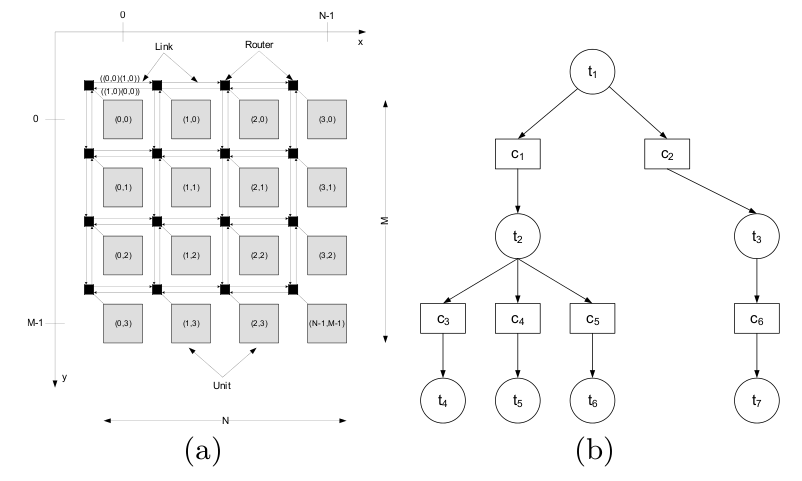
\includegraphics[width=10cm]{images/7}%
\framebox{\begin{minipage}[t]{0.2\columnwidth}%
Fig. 9\cite{Weichslgartner:2011:DDM:1999946.1999979}%
\end{minipage}}


\subsection{The APCG}

The methodology proposed in this paper is tailored for dataflow-dominated
streaming applications, with characteristics typically found in multimedia,
telecommunication, and signal processing. For the analysis presented
in this work, we make following assumptions:

A1: An application $i$ is executed periodically with period $P_{i}$
. 

A2: Data-dependencies between functional blocks result in a tree-shaped
dataflow. 

A3: Applications are characterized by bandwidth-oriented one-to-one
communications between tasks.

A graph-based, formal model of each applications as it is illustrated
in Fig. 9(b) can be given as follows: 

A tree-structured application $i$ is modeled as an acyclic bipartite
$G_{A}$($V_{i}$,$E_{i}$). The set $V_{i}=$$T_{i}+C_{i}$ is a
union of task vertices $T_{i}$and communication vertices $C_{i}$.
The application further satisfies the points discussed in section
4.2.


\subsection{The hardware graph}

HG - As is depicted in Fig 9(a) Each unit consists of one processing
element (PE) and one router that is connected to the local PE (through
a Network-Interface (NI)) and the four routers in the cardinal directions.
Tasks can be loaded and executed on the PEs. Each unit $u\in U$ provides
a limited amount of consumable resources that can be occupied by tasks,
e.g., memory for storing data and program code. This limit is denoted
as res(u). The maximal available bandwidth of a link $l\in L$ is
limited to band(l). 


\subsection{Creating the CTG}

Each task $t$$\in$ $T_{i}$ is characterized by its execution time
$exec(t,u)$ on PE $u\in U$ and the resources required for successfully
executing the task on the PE $req(t,u)$. Each message $c\in C$ is
designated with its payload $size(c)$. 

Once the CTG is created, we will be able to define values like bandwidth
of communication vertex $c$. 

$bw(c)=\frac{size(c)}{P_{i}}$

We will be further able to define values like load imposed by task
$t$ on unit $u$. 

$load(t,u)=\frac{exec(t,u)}{P_{i}}$

Application mapping can now be described as embedding the application
graph onto the NoC graph. This involves a) task mapping and b) communication
routing. Task mapping is denoted as m : $T_{i}$$\rightarrow U$ ,
i.e. , assigning tasks to processing elements. Routing is defined
as 

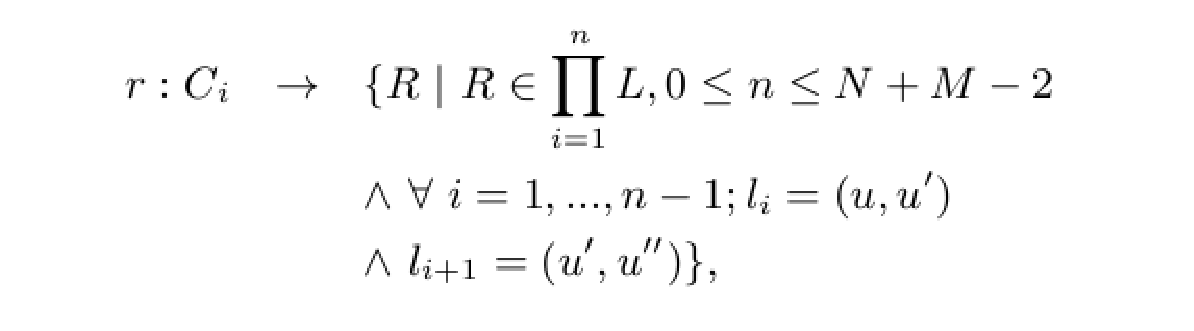
\includegraphics[width=9cm]{images/8}

i.e., each communication node is assigned with a route through communication
links. For example, a route with n hops can be described as a sequence
$r(c_{i})=(l_{1},l_{2}...l_{n})$. A feasible mapping is give, if
the following constraints hold:

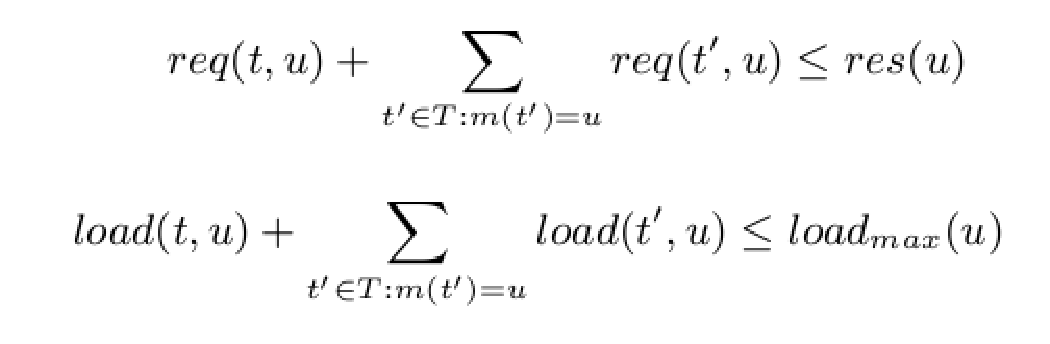
\includegraphics[width=7cm]{images/9}

where first equation ensures that resource restrictions are respected,
and second is the schedulability test of resource u. Moreover, a feasible
routing has to consider the available bandwidth.

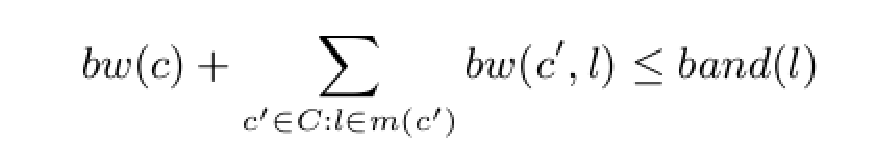
\includegraphics[width=7cm]{images/10}

\textbf{SELF-EMBEDDING ALGORITHM} - is the algorithm used in this
decentralized architecture. As the inspected application topologies
are treestructured, tasks can be embedded incrementally by an already
mapped predecessor task. Only the root nodes have to be placed differently,
since they have no predecessor tasks. There are various methods proposed
in \cite{Weichslgartner:2011:DDM:1999946.1999979} to select this
seed node. Distributing the mapping calculation to the task nodes
helps to parallelize the workload and to prevent a single point of
failure. 

A run example of the above algorithm:

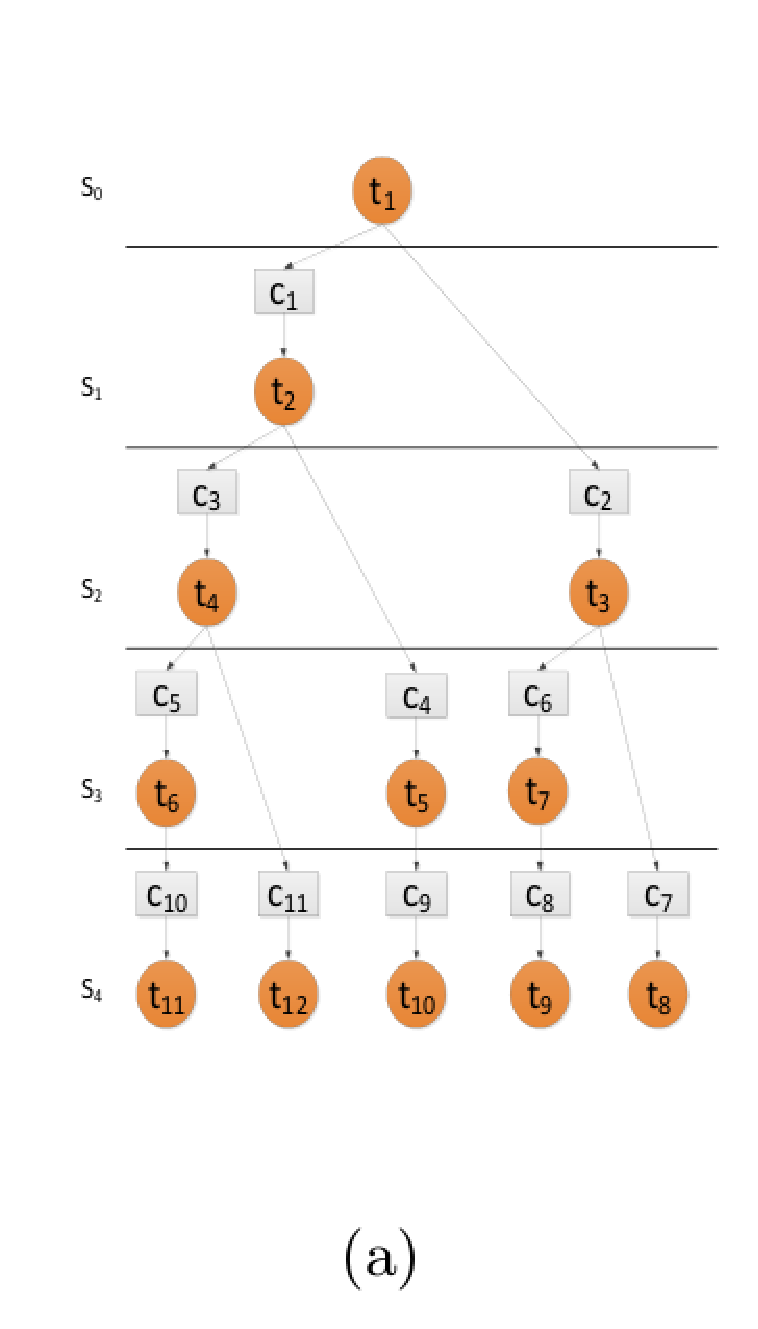
\includegraphics[height=10cm]{images/11}

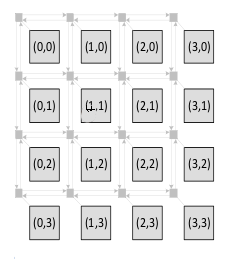
\includegraphics[width=17cm]{images/12}

Figure 10: An example of a self-embedding algorithm with the initial
search space of 1 hop. In the upper half the search space is shown
and in the lower half the mapping. The root node t0 is embedded initial
with the seedpoint selection in mapping step S0 . In mapping step
S1 it starts the embedding algorithm for t2 and c1 . In S2 , it starts
the embedding for t3 and c2 . In the same mapping step, t2 itself
can start the embedding of t4 and c3 , and so on. While embedding
the right successor, the already mapped left successor can embed its
own successors in parallel. 

\ \\

\textbf{SEED POINT SELECTION} 

As every task places its succeeding tasks and communication, the initial
task or root task has to be placed by a different algorithm. For these
tasks, it is necessary to find those units on the NoC on which it
is suitable to load the root nodes. We call these units seed points
($U_{s}$) and several methodologies are available to determine this
set. As we don\textquoteright{}t want to loose the decentralized characteristics
of our approach, the seed point determination should not have a global
view of the entire NoC system. Nevertheless, some global information,
like the size of NoC, previous seed points and cluster information
have to be stored centrally. However, these algorithms are only executed
once per application and the saved information is linear in the NoC
size. So the scalability is kept. 

\textbf{SIMULATION RESULTS}

Authors of the above cited paper have run elaborate simulations and
found that for specific structures (in this case , tree structured
applications), the decentralized algorithms for mapping give results
at par with the centralized ones.


\chapter{Conclusion}

In this report we discussed the various paradigms available for running
real life applications on the NoC architectures. We analysed the reasons
that forced us to make the switch from the currently prevalent architectures.
We established the asymptotic supremacy of NoCs over other architectures.
We saw that the applications need to be mapped before being run on
a multicore. Amongst the various paradigms used for mapping centralized
has been deeply explored till date whereas decentralized has been
ignored for a while. We reasoned that the centralized approach is
not scalable , and that going decentralized is the best way for future.
The recent paper about decentralized mapping of tree structured applications
has shown that with sufficient attention , decentralized mapping mechanisms
can come at par with the centralized ones , thus paving way for a
scalable technology.
}\maketitle


\pagebreak{}


\lhead[]{Acknowledgments}


\rhead[Acknowledgments]{}


\chapter*{Acknowledgments}

\addcontentsline{toc}{chapter}{Acknowledgments} 

I would like to thank Dr. Hemangee Kapoor for her continued support
and guidance.


\pagebreak{}


\lhead[]{\rightmark}


\rhead[\leftmark]{}

\bibliographystyle{alpha}
\bibliography{thesisExample}

\end{document}
